\chapter{Pruebas}

% hacer ya DISEÑO PRUEBAS y diseño interfaz

% primera entre el 2 y 4

% segunda 10




% pruebas de usabilidad, (modificaciones) y de software

% net promoter score
% describir participantes, métricas
% describir resultado de cada tarea

Tras el capítulo anterior, ya tenemos una implementación de nuestra herramienta que los usuarios pueden probar para darnos retroalimentación de cara a mejorar la usabilidad de la plataforma.

Las pruebas que se van a realizar en este trabajo, dado que la metodología usada ha sido la del \textit{Design Thinking} y el Diseño Centrado en el Usuario, serán pruebas de usabilidad con usuarios reales.

\section{Diseño de las pruebas}

En esta sección se va a determinar cuál será el diseño de las pruebas de usabilidad. Para ello debemos concretar quién participará en las pruebas, qué tendrán que hacer y qué se les va a preguntar.

\subsection{Participantes}

Para esta primera versión se harán pruebas con 10 personas.

Dado que hay dos roles claramente distinguibles en la aplicación, se seleccionarán 3 administradores y 7 miembros para completar la prueba de usabilidad.


\subsection{Tareas a realizar}

Para comprobar la usabilidad los flujos de trabajo distintos de administradores y miembros, se van a proponer tareas distintas para cada uno de los dos roles.

En el caso de los administradores:

\begin{enumerate}
    \item Crea una agrupación.
    \item Crea un evento.
    \item Edita la descripción de la agrupación.
    \item Sube una obra a la agrupación.
    \item Invita a un miembro de tu banda.
    \item Haz que no pueda unirse nadie más a la agrupación.
    \item Haz administrador al miembro que se ha unido.
    \item Quítale los permisos de administrador al miembro que se ha unido.
    \item Elimina el evento que creaste.
\end{enumerate}

En el caso de los miembros:

\begin{enumerate}
    \item Únete a una agrupación.
    \item Mira los eventos de la agrupación.
    \item Descarga alguna obra de la agrupación.
    \item Sal de la agrupación.
\end{enumerate}


\subsection{Preguntas a realizar}

Las preguntas que se van a realizar a los usuarios son las descritas en la tabla \ref{tab:preguntasPrueba}.

Las relacionadas con tareas concretas nos ayudarán a realizar una mejora de la usabilidad antes de la entrega, solucionando los problemas que manifiesten los usuarios y que se puedan solucionar rápidamente, y planificando como trabajos futuros las soluciones más costosas.

Por otro lado, la primera pregunta genérica nos ayudará a calcular el \textit{NET Promoter Score} o NPS. Según esta herramienta, los encuestados que respondan entre 0 y 6 son detractores, entre 7 y 8 son pasivos y entre 9 y 10 son promotores. De esta forma, se obtendrá un índice realizando el siguiente cálculo:
\[
\textrm{NET} = \frac{\textrm{Promotores} - \textrm{Detractores}}{\textrm{Encuestados}} \times 100
\]

Este índice puede resultar entre -100 y 100. Diremos que tiene un resultado positivo si es mayor a 0, y excelente si es mayor a 50.


\begin{table}[]
    \centering
    \begin{tabular}{|l|c|}
        \hline
        \multicolumn{2}{|c|}{\textbf{Preguntas por tarea}} \\
        \hline
        \textbf{Pregunta} & \textbf{Tipo de respuesta} \\
        \hline
        1. ?`Has podido realizar la tarea? & Sí/No \\
        \hline
        2. ?`Ha sido fácil realizar la tarea? & Entre 1 y 5. \\
        \hline
        \hline
        \multicolumn{2}{|c|}{\textbf{Preguntas genéricas}} \\
        \hline
        \textbf{Pregunta} & \textbf{Tipo de respuesta} \\
        \hline
        1. ?`Algún comentario sobre las tareas? ?`Errores? & Respuesta libre. \\
        \hline
        2. ?`En qué dispositivo has probado el bot? & \makecell{Móvil / \\Ordenador con aplicación / \\ Ordenador en Telegram Web / \\ Otro} \\
        \hline
        3. ?`Opinión sobre la web \texttt{mordente.es}? & \makecell{Entre 0 y 5 para \\ información, diseño adaptativo,\\ apariencia y velocidad} \\
        \hline
        4. ?`Recomendarías Mordente a un amigo? & Entre 0 y 10 \\
        \hline
        5. ?`Tienes algún comentario genérico? & Respuesta libre. \\
        \hline
    \end{tabular}
    \caption{Formulario para la prueba de usabilidad}
    \label{tab:preguntasPrueba}
\end{table}

\section{Realización de las pruebas}


\section{Informe final de las pruebas}


\subsection{Problemas detectados}

\subsubsection{\texttt{username} vacío}

Uno de los problemas detectados durante las pruebas viene derivado por el hecho de que Telegram no obliga a los usuarios a asignarse un nombre de usuario, por lo que el campo \texttt{username} de nuestra base de datos se queda vacío. Esto resultaba en una excepción controlada a la hora de actualizar sus datos que se ha corregido\footnote{\url{https://github.com/daniharo/mordente/commit/70b3b54}}.

\subsubsection{Desbordamiento del campo de ID de Telegram}

Uno de los usuarios que realizaron las pruebas se puso en contacto para manifestar que no era capaz de obtener ninguna respuesta por parte del bot: siempre obtenía un mensaje de error.

Revisando \textbf{Sentry} (sección \ref{subsection:sentry}), vemos que se ha registrado el error (figuras \ref{fig:sentryListaErrores} y \ref{fig:sentryDetalleError}) y que se debe a que el ID de Telegram del usuario no cabe en el tipo \texttt{INTEGER} de \textbf{PostgreSQL}. Revisando la documentación de Telegram\footnote{\url{https://core.telegram.org/bots/api\#chat}}, descubrimos efectivamente que los IDs de Telegram pueden ocupar hasta 52 bits, mientras el tipo \texttt{INTEGER} alberga hasta 32 bits incluyendo el signo.

Para solucionar el problema, migramos la columna \texttt{uid} de la tabla \texttt{User} al tipo \texttt{Float} de Prisma\footnote{\textit{Commit:} \url{https://github.com/daniharo/mordente/commit/46f665c0}}, de forma que el usuario ya pudo terminar las pruebas correctamente.

\begin{figure}[h]
\centering
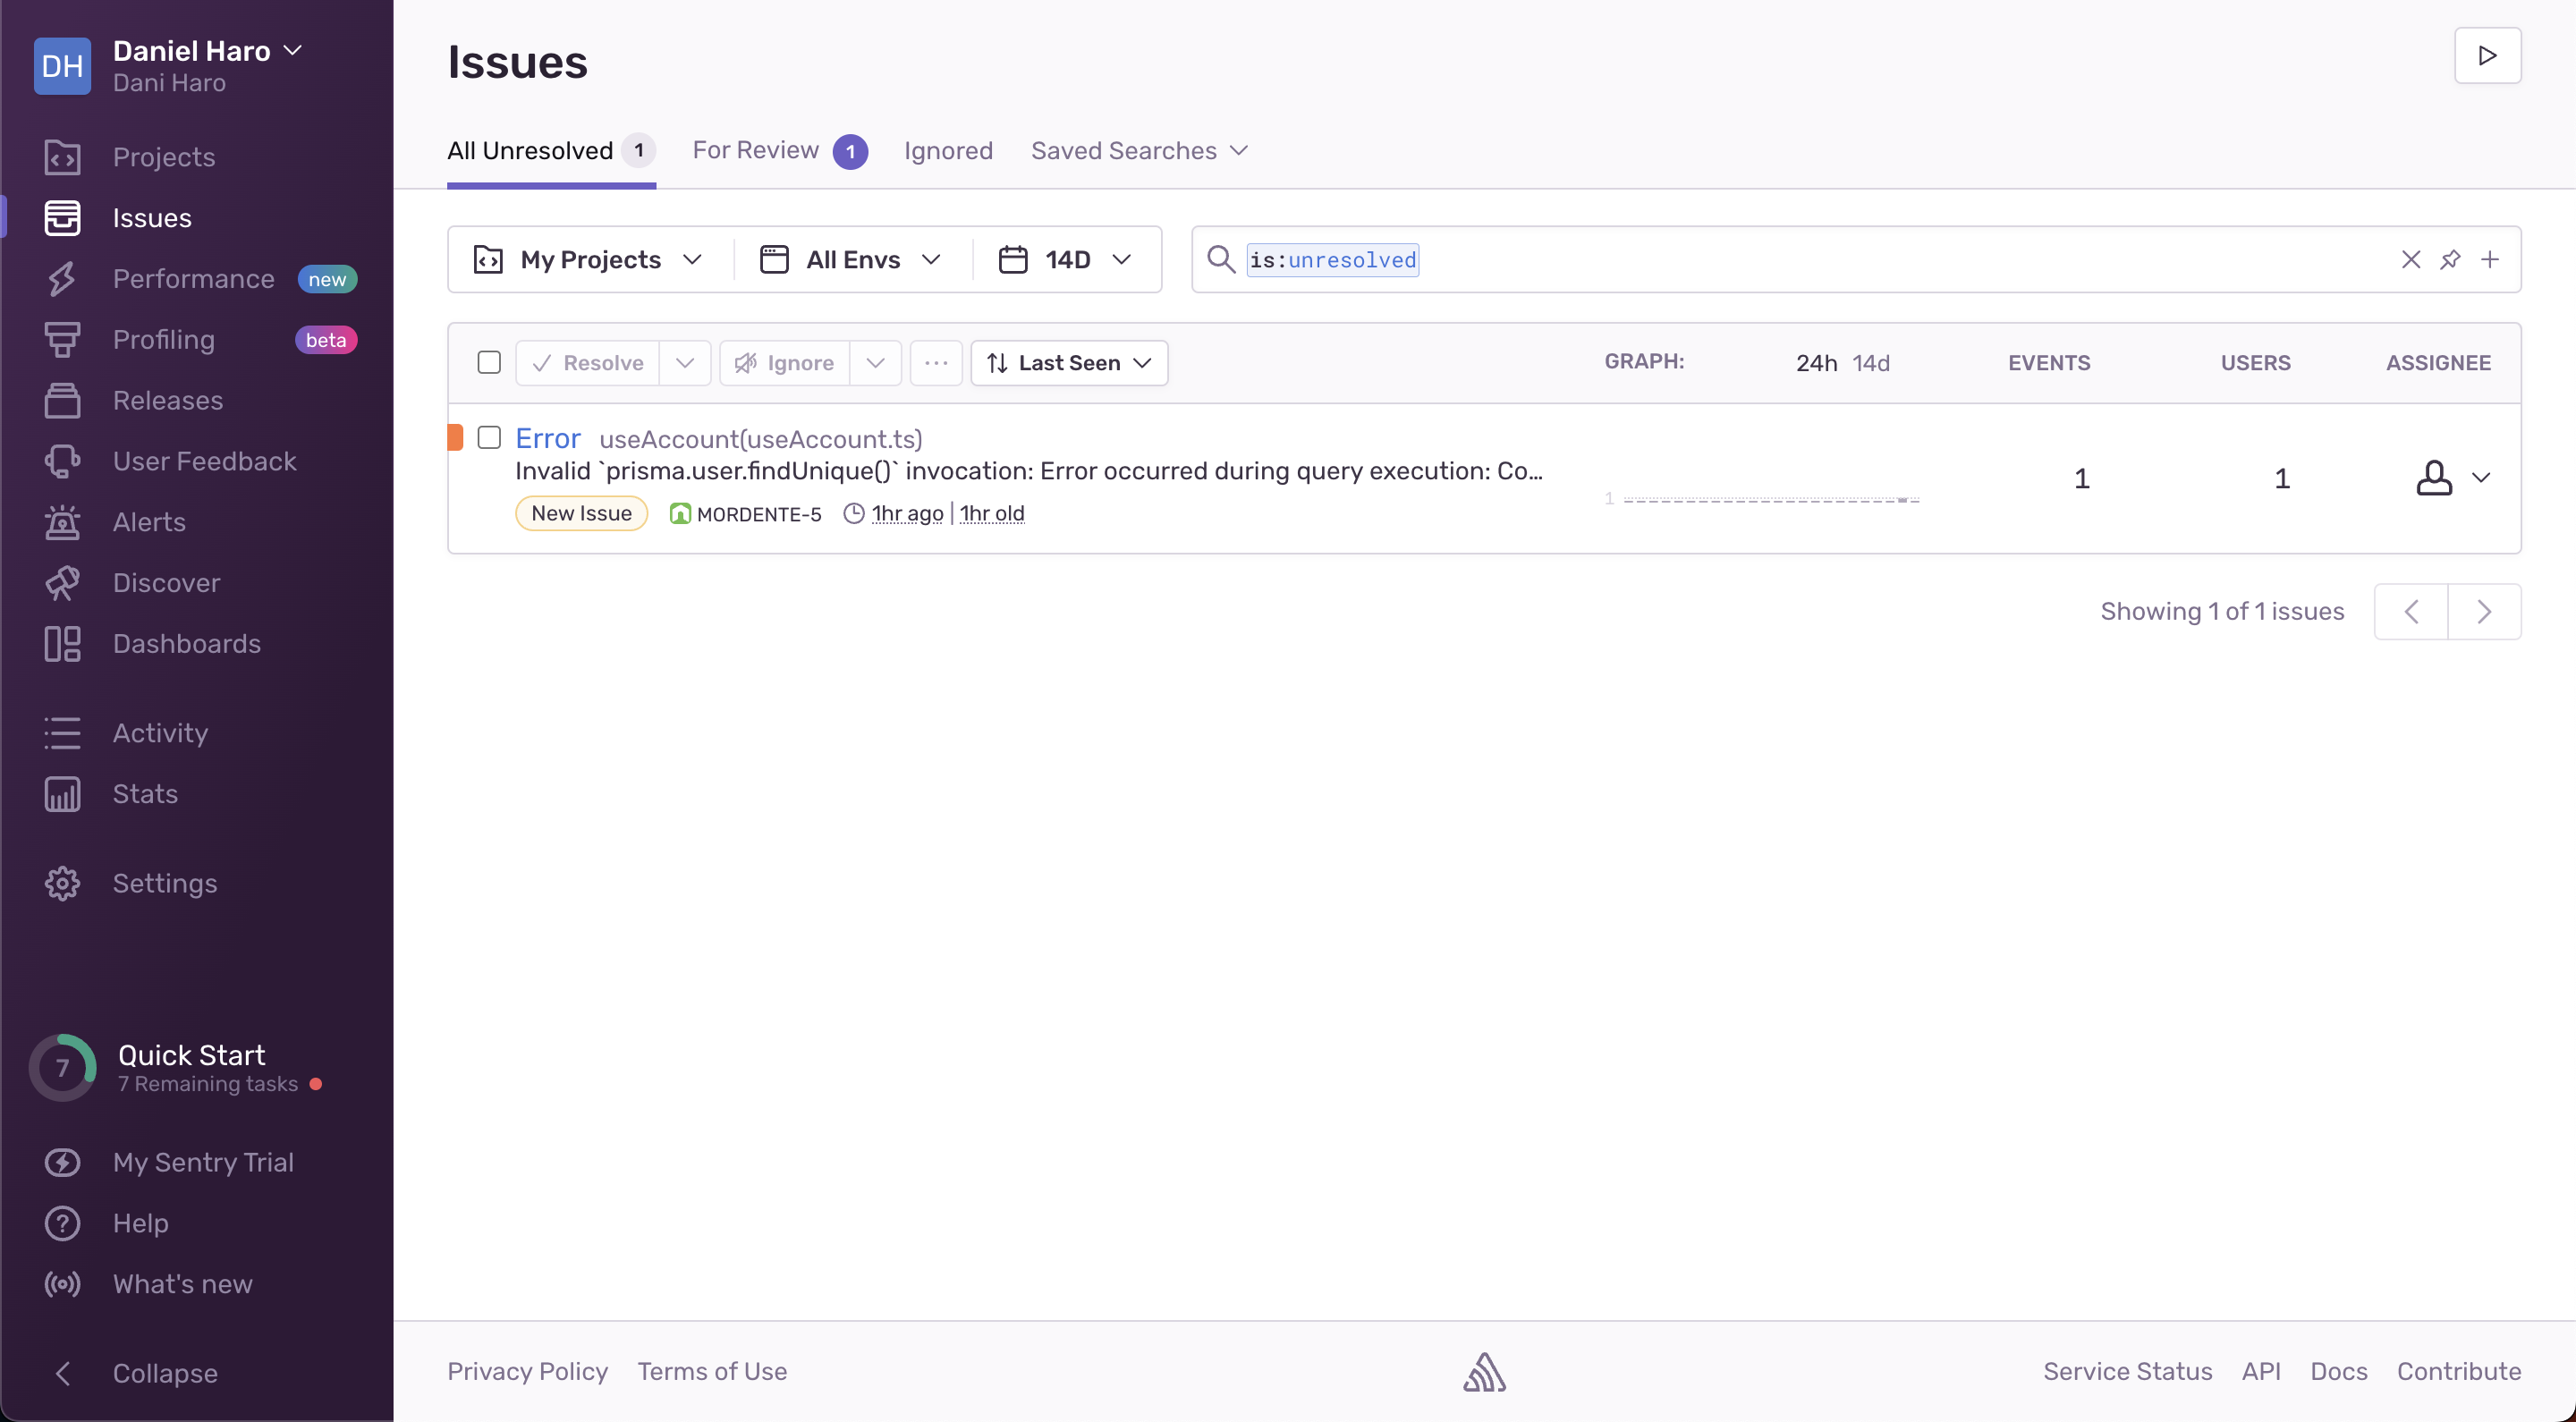
\includegraphics[width=0.75\textwidth]{imagenes/pruebas/sentry_error_uid.png}
\caption{Lista de errores registrados en Sentry}
\label{fig:sentryListaErrores}
\end{figure}

\begin{figure}[h]
\centering
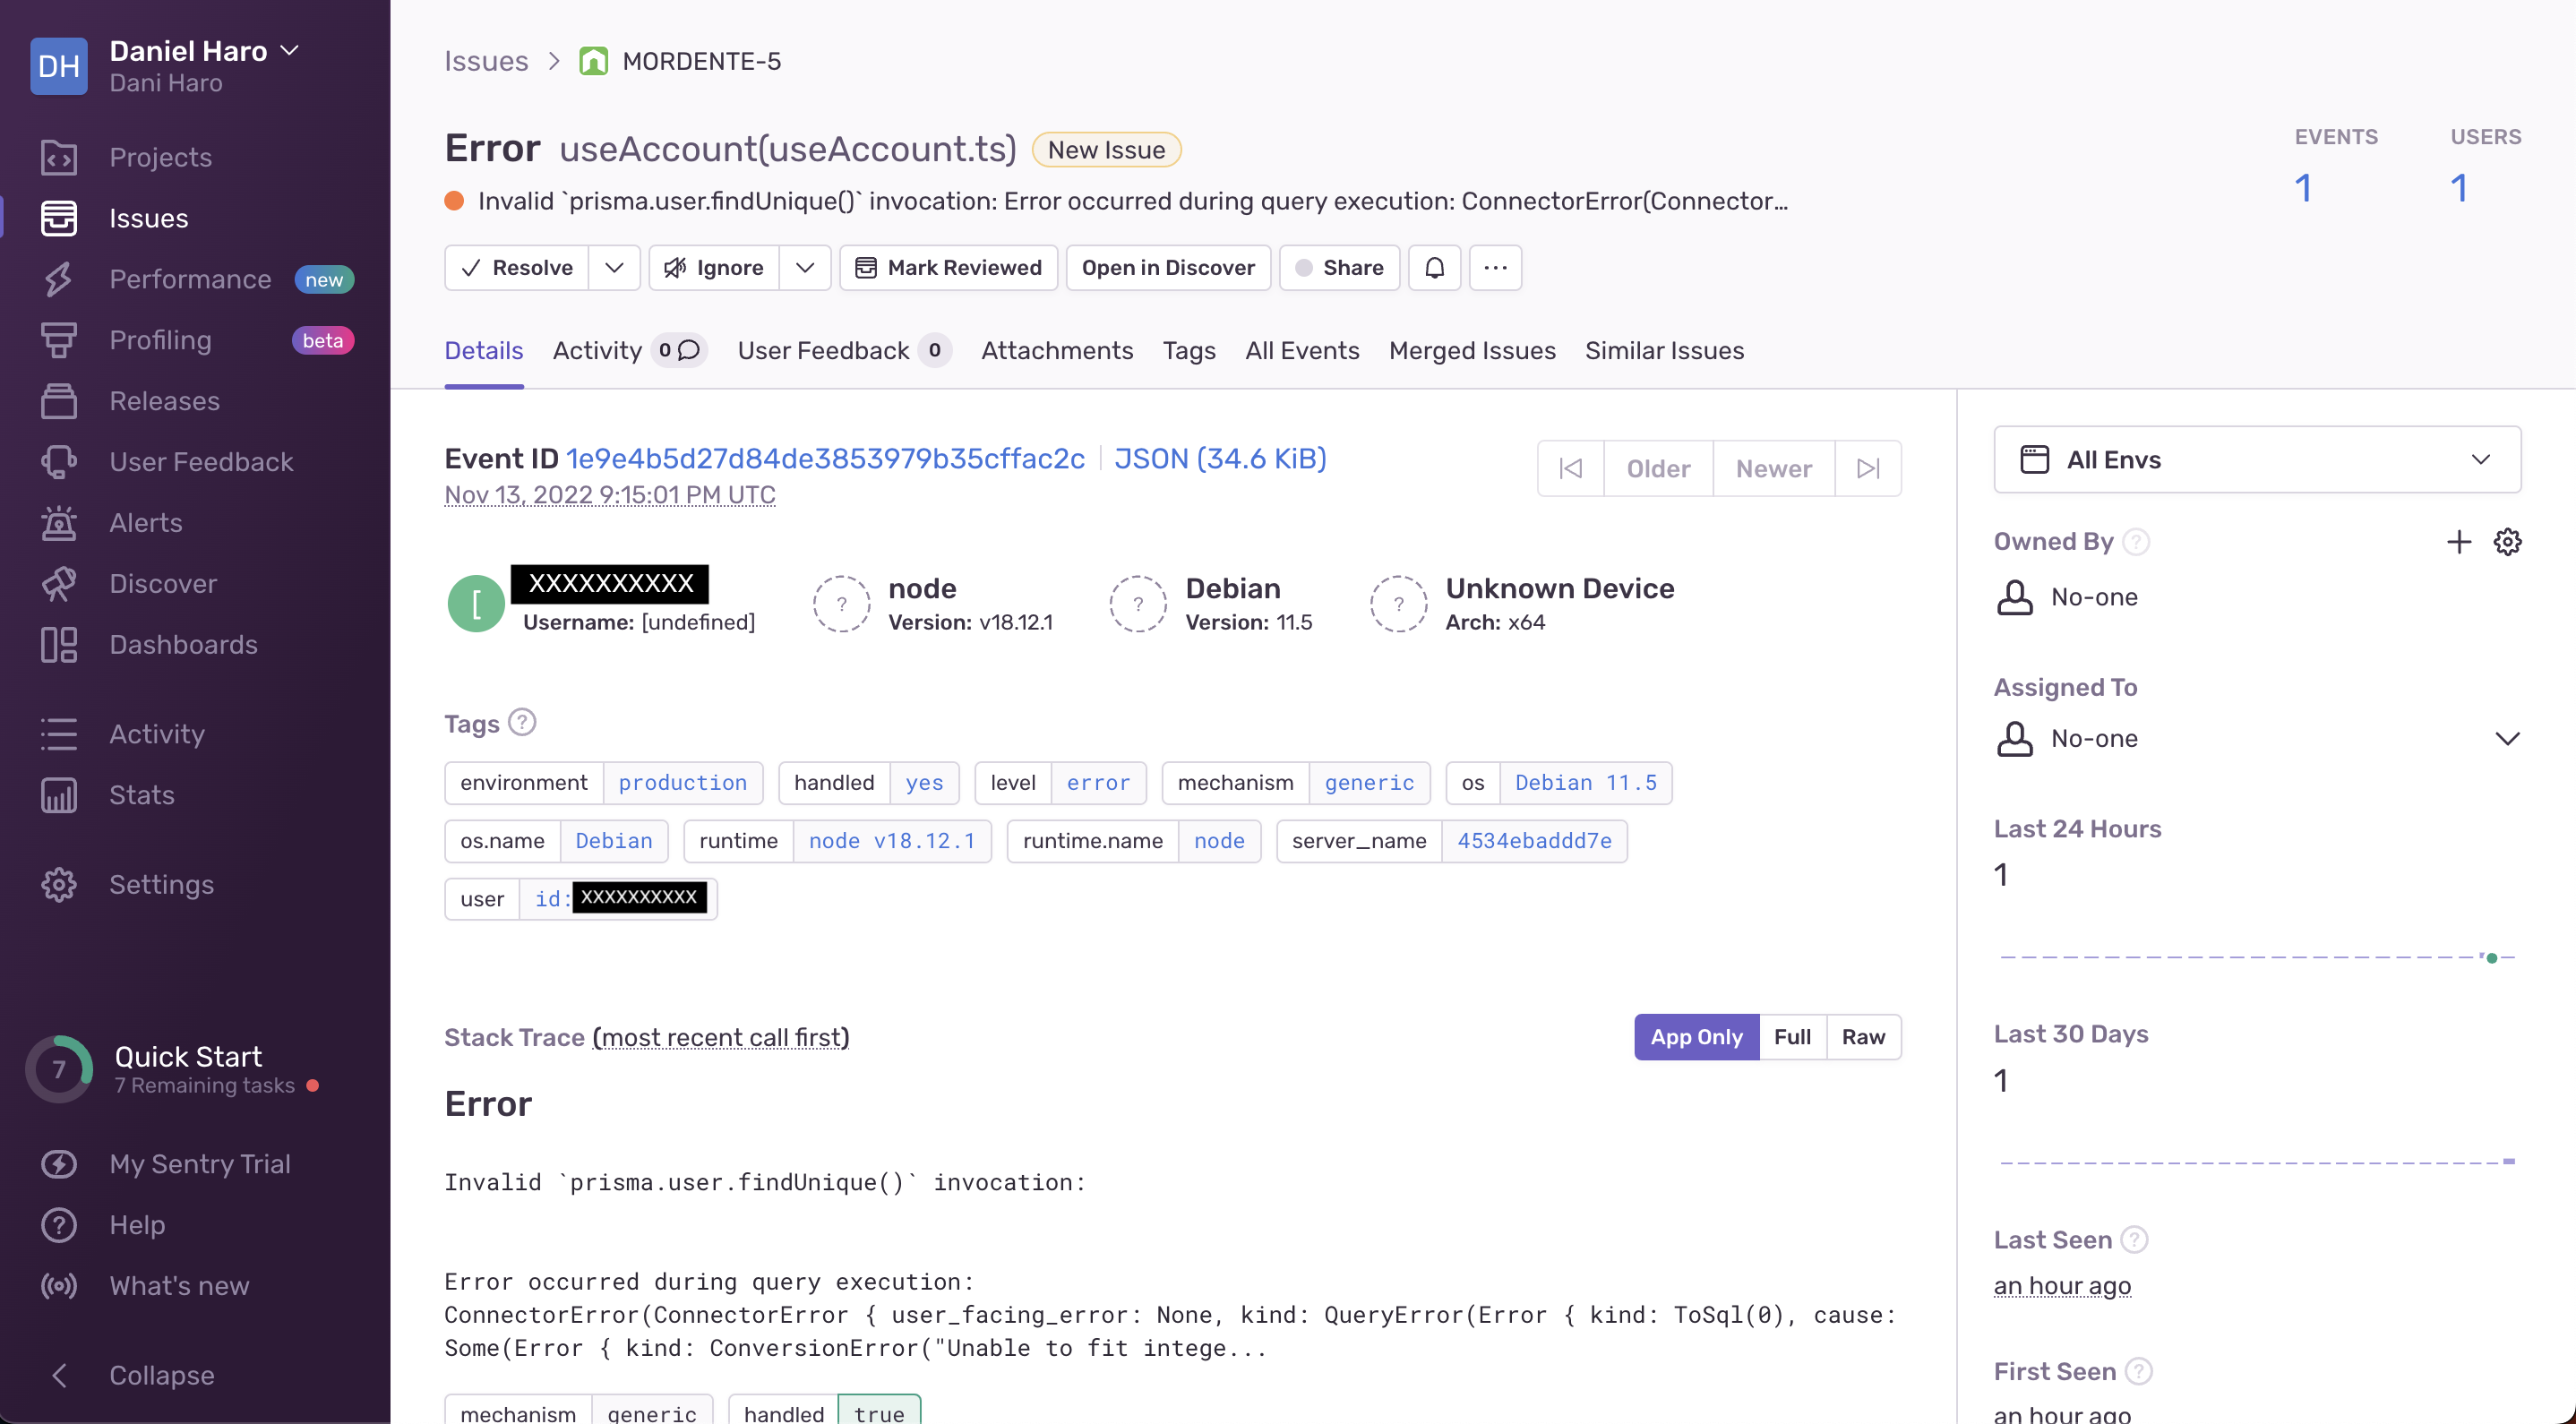
\includegraphics[width=0.75\textwidth]{imagenes/pruebas/sentry_detalle_error_uid.png}
\caption{Detalle del error generado por desbordamiento del ID de Telegram}
\label{fig:sentryDetalleError}
\end{figure}

\subsection{Peticiones}

Una de las peticiones más populares ha sido la de incorporar la funcionalidad de \textbf{calendario} ya que la alternativa que se ha analizado en la sección \ref{subsection:glissandoo} no la implementa. Dado que requiere de más esfuerzo para su implementación, se ha programado como trabajo futuro.


\section{Demostración en vídeo}

Se puede visualizar el funcionamiento del bot en el vídeo disponible en este enlace:
\url{}

